\documentclass{article}
\usepackage{polski}
\usepackage[utf8]{inputenc}
\usepackage{graphicx}
%s\usepackage[margin=2.5cm]{geomtry}

\usepackage{graphicx}    % Pakiet pozwalający ,,wklejać'' grafikę...
\usepackage{subcaption}
\usepackage{amsmath,amssymb,amsfonts,amsthm,mathtools}
                               % Dołączamy zestaw różnych przydatnych znaczków ...
\DeclareMathOperator{\arccosh}{arccosh}
% dane autora
\author{Wiktor Pilarczyk}
\title{Pracownia z analizy numerycznej\\\small{Zadanie: P2.2}\\\large{Prowadzący: Witold Karczewski}}
\date{\today}
% początek dokumentu
\begin{document}
\maketitle
\section{Aproksymacja}
Aproksymacja jak sama nazwa wskazuje polega na przybliżaniu, pojęcie to jest głównie związane z funkcjami, które można przybliżać za pomocą prostszych funkcji (latwiejszych do obliczenia lub zawierających mniej informacji). W informatyce oraz wielu dziedzinach pokrewnych częstym problemem są ograniczone zasoby (np. pamięć lub moc procesora), przez co zamiast obliczania dokładnego wyniku, zadowalająca jest jego aproksymacja, która nieznacznie się różni. Jeśli już przybliżamy funkcję to chcemy, aby była optymalna, czyli aby przy korzystaniu z tych samych zasobów było to najlepsze oszacowanie wyniku.

\subsection{Podstawowe definicje i własności}
Definicja iloczynu oraz normy, która wyraża się poprzez ten iloczyn pozwala zdefiniować przestrzeń liniową (unitarną), dzięki której znalezienie elementu optymalnego sprowadza się do rozwiązania układu liniowego.
Podstawowe własności iloczynu skalrnego:
\begin{tabbing}
\quad a)  $< f,g > \ = \ <g,f>$\\
\quad b)  $<f, \alpha g + \beta h> \ = \ <f, \alpha g> + <f, \beta h>$\\
\quad c)  $<f,f> \ \geq \ 0$  
\end{tabbing}
Jeśli f $\in \mathrm{E}$ i g $\in \mathrm{G}$, gdzie E jest przestrzenią unitarną, a G jest jej podprzestrzenią to $w^{*} \in \mathrm{G}$ najlepiej aproksymuje f (jest elementem optymalnym), gdy: 
\begin{equation} 
    \| f - w^{*} \| = dist(f,G) = inf_{g \in G} \ \| f - g \|
\end{equation}
Dla każdej podprzestrzeni skończeniowymiarowej G istnieje punkt optymalny (Kincaid 367) oraz w jest optymalny $\Leftrightarrow \ f - w^{*} \  \perp \  G $ (Kincaid 369).\\
Baza ortogonalna $ \{ B_{i} \}$ jest to zbiór wektorów z przestrzeni unitarnej, która ma następujace własności:
\begin{tabbing}

\quad a)  $< B_{i},B_{j} > \ = \ 0 \  \ i \neq j $\\
\quad b)  $ \forall_{f \in E} \ \ f = \sum_{i=1}^{\infty} \alpha_{i} B_{i}$
\end{tabbing}
więc dowolny f $\in$ E można przedstawić za pomocą sumy wektorów bazy.
\newpage
\section{Aproksymacja średniokwadratowa na zbiorze dyskretnym}
\subsection{Iloczyn skalarny na zbiorze dyskretnym}
Jeśli mamy zbiór n + 1 punktów $\{ x_{i} \} $ gdzie $\ i \in \mathbb{N}$ \ oraz \ $ i \leq n$, jak również funkcje f i g, dla których znane są wartości w punktach $\{x_{i}\}$ definiujemy iloczny skalarny:
\begin{equation}
    < f,g > = \sum_{i=0}^{n}f(x_{i})g(x_{i})
\end{equation}

\begin{proof}
Sprawdzamy czy (2) spełnia definicję iloczynu skalranego.\\
\begin{tabbing}
\quad a)  Weżmy dowolne f i g dla zbioru n + 1 elementowego punktów $\{ x_{i} \}$. \\ \\
\qquad $< f,g > \ = \ \sum_{i=0}^{n}f(x_{i})g(x_{i}) \ = \ \sum_{i=0}^{n}g(x_{i})f(x_{i}) \ = \ < g,f >$\\\\
\quad b)  Weżmy dowolne $\alpha i \beta \in \mathbb{R}$ f, g i h dla zbioru n + 1 elementowego punktów $\{ x_{i} \}$. \\ \\
\qquad  $<f, \alpha g + \beta h> \  = \ \sum_{i=0}^{n}f(x_{i}) \ (\alpha g(x_{i}) + \beta h(x_{i})) \ =$ \\ \\ 
\qquad $= \sum_{i=0}^{n}f(x_{i}) \ \alpha g(x_{i}) + \sum_{i=0}^{n}f(x_{i}) \ \beta h(x_{i}) \ = \ <f, \alpha g> + <f, \beta h>$\\ \\ 
\quad c)  Weżmy dowolne f dla zbioru n + 1 elementowego punktów $\{ x_{i} \}$. \\ \\
\qquad $ <f,f> = \sum_{i=0}^{n}f(x_{i})f(x_{i}) = \sum_{i=0}^{n}f(x_{i})^{2} \geq 0$
\end{tabbing}
\end{proof}
\subsection{Wielomian optymalny na zbiorze dyskretnym}
Niech $\{B_{i}\}$ będzie bazą dla $\Pi_{k}$. Spróbujmy znaleźć wielomian optymalny $w_{k}^{*}$ k-tego stopnia dla dowolnej funkcji f, która jest określona dla zbioru n + 1 elementowego punktów $\{ x_{i} \}$.\\
Ponieważ $\{B_{i}\}$ jest bazą więc $w_{k}^{*} = \sum_{i=0}^{k} \alpha_{i}B_{i}$, więc dla dowolnego i otrzymujemy równanie:
\begin{equation}
    < f - w_{k}^{*}, B_{i} > = <f, B_{i}> - <w_{k}^{*}, B_{i} >
\end{equation}
z (1) otrzymujemy:
\begin{equation}
    <f, B_{i}> - <w_{k}^{*}, B_{i} > = 0
\end{equation}
przekształcajać równanie:
\begin{equation}
    <f, B_{i}> = \sum_{j=0}^{k} \alpha_{i} < B_{j},B_{i}>
\end{equation}
więc otrzymujemy wzór na $\alpha_{i}$:
\begin{equation}
    \alpha_{i} = frac{<f, B_{i}>}{\sum_{j=0}^{k} < B_{j},B_{i}>}
\end{equation}
Skoro dla każdego i otrzymujemy równanie (5), możemy stworzyć układ równań i zapisać je w macierzy:\\\\
\begin{equation}
\begin{pmatrix}
  <B_{0},B_{0}> & <B_{1},B_{0}> & \cdots & <B_{k},B_{0}> \\
  <B_{0},B_{1}> & <B_{1},B_{1}> & \cdots & <B_{k},B_{1}> \\
  \vdots  & \vdots  & \ddots & \vdots  \\
  <B_{0},B_{k}> & <B_{1},B_{k}> & \cdots & <B_{k},B_{k}> 
 \end{pmatrix}
\begin{bmatrix}
    \alpha_{0} \\
    \alpha_{1} \\
    \vdots  \\
    \alpha_{k} \\
  \end{bmatrix} 
  =
  \begin{bmatrix}
    <f, B_{0}>  \\
    <f, B_{1}>  \\
    \vdots  \\
    <f, B_{k}>  \\
  \end{bmatrix} 
\end{equation}
Więc
Jeśli baza jest ortogonalna wtedy $<B_{i},B_{j} = 0$ dla $i \neq j$, więc otrzymujemy macierz diagonalną:
\begin{equation}
\begin{pmatrix}
  <B_{0},B_{0}> & 0 & \cdots & 0 \\
  0 & <B_{1},B_{1}> & \cdots & 0 \\
  \vdots  & \vdots  & \ddots & \vdots  \\
  0 & 0 & \cdots & <B_{k},B_{k}> 
 \end{pmatrix}
\begin{bmatrix}
    \alpha_{0} \\
    \alpha_{1} \\
    \vdots  \\
    \alpha_{k} \\
  \end{bmatrix} 
  =
  \begin{bmatrix}
    <f, B_{0}>  \\
    <f, B_{1}>  \\
    \vdots  \\
    <f, B_{k}>  \\
  \end{bmatrix} 
\end{equation}
Więc dla każdego i otrzymujemy układ równań:
\begin{equation}
<f, B_{i}> \ = \ \alpha_{i} < B_{i},B_{i}>
\end{equation}
Co umożliwia łatwe wyliczenie wielomianu optymalnego, gdyż korzystając z (8) oraz własności bazy ortogonalnej otrzymujemy:
\begin{equation}
w_{k}^{*} = \sum_{i=0}^{k} \alpha_{i}B_{i} = \sum_{i=0}^{k} \frac{<f,B_{i}>}{<B_{i},B_{i}>}B_{i}
\end{equation}
\subsection{Obliczanie bazy ortogonalnej}
Do obliczenia bazy ortogonalnej skorzystamy z zależności rekurencyjnej:
$$P_{0}(x) = 1 \ \ \ \ \ \ \ \ \ \ \ \ P_{1}(x) = 1 - a_{1}$$
\begin{equation}
P_{k}(x) = (x - a_{k}) P_{k-1}(x) - b_{k}P_{k-2}(x)
\end{equation}
gdzie
$$a_{k} = \frac{<xP_{k-1},P_{k-1}>}{<P_{k-1},P_{k-1}>} \ \ \ \ \ \ b_{k} = \frac{<P_{k-1},P_{k-1}>}{<P_{k-2},P_{k-2}>}$$
\newpage
\subsection{Postać potęgowa wielomianu}
Przy szukaniu wielomianu optymalnego wystarczy spamiętywać wartości w podanych punktach $x_{i}$, aby wyliczyć jego postać skorzystamy z uogólnionego algorytmu Clenshawa, wymaga to spamiętywania współczynników: $\alpha_{i}$, $a_{i}$ oraz $b_{i}$.\\
Dla bazy zadanej powyżej (10), algorytmu Clenshawa przyjmuje postać:
$$V_{k} = \alpha_{k} + (x - a_{k+1})V_{k+1} - b_{k+2}V_{k+2}$$
gdzie
$$V_{n+1} = V_{n+2} = 0$$
wtedy
$$w_{n}^{*} = V_{0}$$
\newpage
\section{Obliczenia}

\subsection{Funkcja $x^5$}
Stopień wielomianu optymalnego,a wielkość $\delta$
\begin{center}
    \begin{tabular}{ |p{3cm}|p{4.6cm}|p{4.6cm}|}
     \hline
     Stopień wielomianu optymalnego & $\delta$ dla punktów równoodległych & $\delta$ dla punktów różnoodległych\\
     \hline
     1 & 1800000 & 1800000\\
     \hline
     2 & 140000 & 10000\\
     \hline
     3 & 1900 & 1\\
     \hline
     4 & 0.000001 & 0.000001\\
     \hline
    \end{tabular}
\end{center}
Wielomian 4 stopnia jest wielomianem interpolacyjnym dla zadanych punktów, dzięki czemu delta może być minimalna (nie może być równa zero, ponieważ wiąże się to z błędem obliczania wartości wielomianu w zadanych punktach).
\begin{figure}[h]
\centering
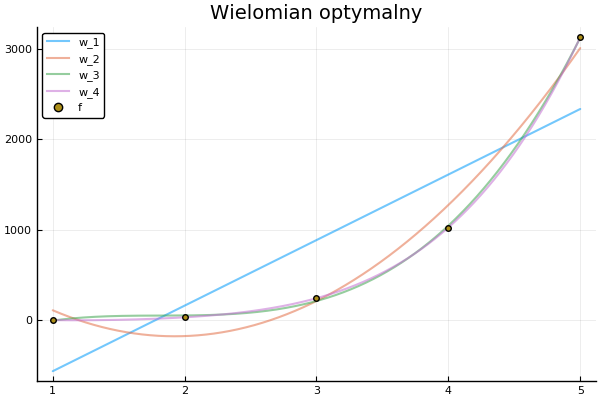
\includegraphics[width=11cm,height=4.91cm]{xpot5.png}
\caption{Dla punktów równoodległych}
\end{figure}

\begin{figure}[h]
\centering
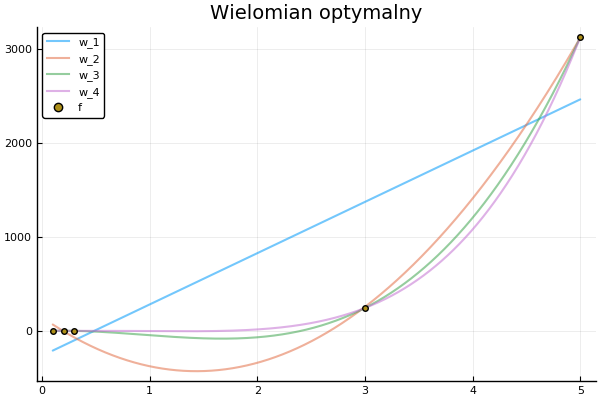
\includegraphics[width=11cm,height=4.91cm]{xpot52.png}
\caption{Dla punktów różnoodległych}
\end{figure}

\subsection{Funkcja $x^{x sin(x)}$}

Stopień wielomianu optymalnego,a wielkość $\delta$
\begin{center}
    \begin{tabular}{ |p{3cm}|p{4.6cm}|p{4.6cm}|}
     \hline
     Stopień wielomianu optymalnego & $\delta$ dla punktów równoodległych & $\delta$ dla punktów różnoodległych\\
     \hline
     0 & 19 & 5\\
     \hline
     1 & 12 & 0.6\\
     \hline
     2 & 9 & 0.2\\
     \hline
     3 & 3 & 0.02\\
     \hline
    \end{tabular}
\end{center}
Delta dla punktów różnoodległych, które można podzielić na podzbiory, wokół jednego punktu jest znacznie mniejsza od delty dla punktów równoodległych dla tego samego zakresu.
\begin{figure}[h]
\center
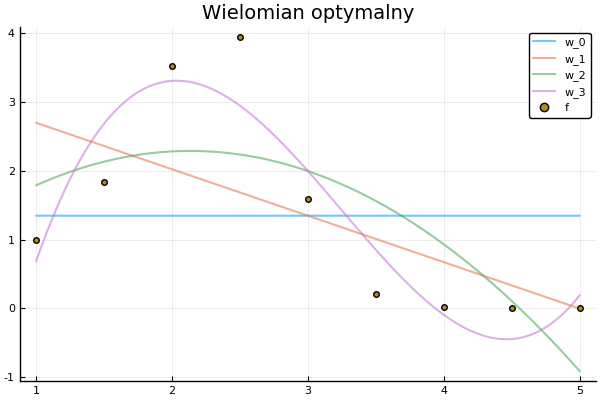
\includegraphics[width=11cm,height=5.3cm]{xpotxsin1.png}
\caption{Dla punktów równoodległych}
\end{figure}

\begin{figure}[h]
\centering
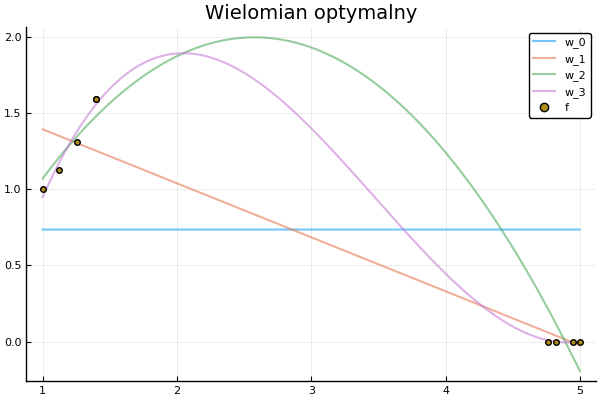
\includegraphics[width=11cm,height=5.3cm]{xpotxsin2.png}
\caption{Dla punktów różnoodległych}
\end{figure}

\subsection{Funkcja $sin(x)$}
Stopień wielomianu optymalnego,a wielkość $\delta$
\begin{center}
    \begin{tabular}{ |p{3cm}|p{4.6cm}|p{4.6cm}|}
     \hline
     Stopień wielomianu optymalnego & $\delta$ dla punktów równoodległych & $\delta$ dla punktów różnoodległych\\
     \hline
     0 & 0.0002 & 0.1\\
     \hline
     1 & 0.0000000000001 & 0.001\\
     \hline
    \end{tabular}
\end{center}
Delta dla punktów równoodległych jest znacznie mniejsza, ponieważ wartości w tych punktach nieznacznie się różnią. 
\begin{figure}[h]
\center
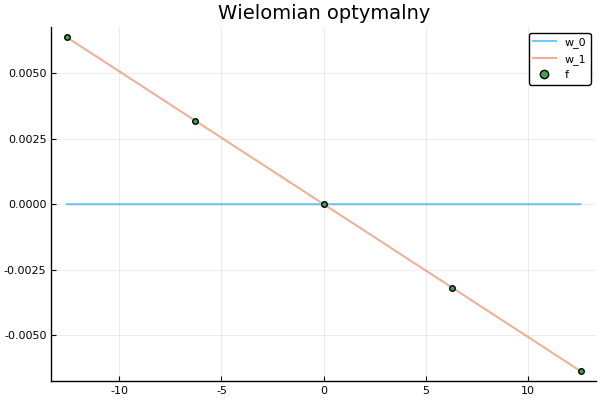
\includegraphics[width=11cm,height=5.8cm]{sin.png}
\caption{Dla punktów równoodległych}
\end{figure}

\begin{figure}[h]
\centering
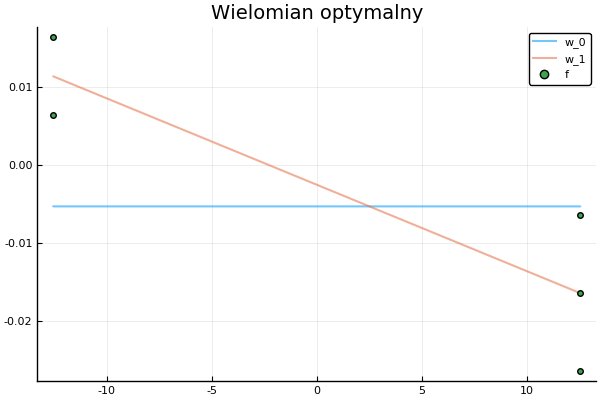
\includegraphics[width=11cm,height=5.8cm]{sin2.png}
\caption{Dla punktów różnoodległych}
\end{figure}
\section{Analiza wyników}
\subsection{Stopień wielomianu optymalnego}
Im zadana delta jest mniejsza tym stopień wielomianu jest większy, wynika to z tego iż im mniejszy błąd chcemy otrzymać tym dokładniejsza musi być aproksymacja. Na podstawie przykładu dla funkcji $x^5$ można też wywnioskować, iż dla wystarczająco małej delty stopień wielomianu optymalnego  będzie równy liczbie punktów minus jeden, wtedy otrzymany wielomian optymalny jest też wielomianem interpolacyjnym dla zadanego zbioru.

\subsection{Rozmieszczenie punktów}
Istotny wpływ ma też odległość między zadanymi punktami, ponieważ im odległość między nimi jest bliższa tym większe prawdopodobieństwo, że wartość funkcji w tych punktach będzie do siebie zbliżona. Dla zbiorów, które składają się z mniejszych podzbiorów oscylujących wokół jednego punktu jest wyższe prawdopodobieństwo, że błędy dla wielomianów optymalnych zadanego stopnia będą niższe niż dla zbioru punktów równoodległych - własność tą można zaobserwować na przykładzie dla funkcji $x ^{x sin(x)}$.
Istnieją przypadki dla, których to stwierdzenie nie jest spełnione, dla powyższego przykładu z $sin(x)$, skorzystano z okresowości sinusa, dlatego funkcja miała zbliżone wartości w równoodległych punktach stąd wartość delty znacząco się różniła od punktów różnoodległych na tym samym przedziale.

\begin{thebibliography}{99}
\bibitem{} D. Kincaid, W. Cheney:
\emph{Analiza numeryczna, WNT, 2005},
\bibitem{} G. Dahlquist, A. Bjorck:
\emph{Numerical Methods in Scientific Computing, Vol.I, SIAM, 2008.},
\bibitem{} M. Dryja, J. i M. Jankowscy:
\emph{Przegląd metod i algorytmów numerycznych cz. 2, WNT, 1988},

\end{thebibliography}

\end{document}

